\documentclass[12pt]{article}

% -----------------------------------------------------------------------
%  Packages
% -----------------------------------------------------------------------
\usepackage[margin=1in]{geometry}
\usepackage{amsmath,amssymb,amsthm}
\usepackage{mathtools}
\usepackage{bm}
\usepackage{graphicx}
\usepackage{booktabs}
\usepackage{array}
\usepackage{caption}
\usepackage{hyperref}
\usepackage[numbers,sort&compress]{natbib}
\usepackage{microtype}
\usepackage{xcolor}
\usepackage[normalem]{ulem}
\usepackage{enumitem}
\usepackage{tikz}
\usetikzlibrary{arrows.meta,positioning}
% Visible revision markup for this review pass. Remove \added/\deleted wrappers
% (and the ulem package) after the changes have been accepted.
\newcommand{\added}[1]{\textcolor{blue!70!black}{#1}}
\newcommand{\deleted}[1]{\textcolor{red!75!black}{\sout{#1}}}
\newcommand{\tbd}[1]{%
  \par\smallskip
  \noindent\fcolorbox{yellow!45!black}{yellow!10}{%
    \parbox{\dimexpr\linewidth-2\fboxsep-2\fboxrule\relax}{%
      \small\textbf{\textsf{TBD}}\enspace\textsf{#1}}}%
  \par\smallskip
}

% -----------------------------------------------------------------------
%  Theorem environments
% -----------------------------------------------------------------------
\theoremstyle{definition}
\newtheorem{definition}{Definition}[section]
\newtheorem{proposition}{Proposition}[section]
\newtheorem{theorem}{Theorem}[section]
\newtheorem{corollary}{Corollary}[section]
\newtheorem{remark}{Remark}[section]
\newtheorem{example}{Example}[section]
\newtheorem{algorithm}{Algorithm}

% -----------------------------------------------------------------------
%  Math macros
% -----------------------------------------------------------------------
\newcommand{\cS}{\mathcal{S}}
\newcommand{\cA}{\mathcal{A}}
\newcommand{\cO}{\mathcal{O}}
\newcommand{\cP}{\mathcal{P}}
\newcommand{\cZ}{\mathcal{Z}}
\newcommand{\cL}{\mathcal{L}}
\newcommand{\cI}{\mathcal{I}}
\newcommand{\cF}{\mathcal{F}}
\newcommand{\cM}{\mathcal{M}}
\newcommand{\cC}{\mathcal{C}}
\newcommand{\cX}{\mathcal{X}}
\newcommand{\E}{\mathbb{E}}
\newcommand{\R}{\mathbb{R}}
\newcommand{\Prob}{\mathbb{P}}
\newcommand{\argmax}{\operatorname{arg\,max}}
\newcommand{\given}{\,\vert\,}

% -----------------------------------------------------------------------
%  Metadata
% -----------------------------------------------------------------------
\title{\textbf{LLM-Grounded User Intent as Action Constraints\\
in Markov Decision Processes}}

\author{Parag Kulkarni\\[4pt]
  \small Opus Technologies\\
  \small \texttt{parag.kulkarni@opustechglobal.com}
  \and
  Baljeet Saini\\[4pt]
  \small Tata Consultancy Services Limited\\
  \small \texttt{Baljeet.Saini@tcs.com}
}

\date{July 2026}

% -----------------------------------------------------------------------
\begin{document}
\maketitle

% -----------------------------------------------------------------------
\begin{abstract}
An autonomous agent acting on a user's behalf must obey explicit instructions
throughout a sequential decision process. Maximizing a reward that captures
average desirability is not sufficient when some actions are prohibited.
Constrained Markov Decision Processes (CMDPs) express restrictions as expected
cumulative costs. A zero-budget CMDP can encode certain zero-violation
requirements, but the user's instruction must first be represented as costs
and thresholds.

We \deleted{study}\hspace{0.25em}\added{present} an \emph{Intent-Constrained Markov Decision Process} (ICMDP), in
which a state-dependent set specifies the actions permitted by the user's
intent. Provided that the specification is correct, the relevant state is
available, and the filter is enforced, an ICMDP policy assigns zero
probability to excluded actions. We give the restricted Bellman equations and
feasibility conditions, \deleted{prove contraction of the Bellman operator,}
\added{record the standard contraction property inherited from
state-dependent-action MDPs,} and show how statewise admissibility can also be
encoded as a zero-budget CMDP. \deleted{Value iteration, policy iteration, and
action-masked model-free methods require only that optimization and exploration
be restricted to admissible actions. A large language model serves as a parser
rather than an enforcement mechanism: it maps an instruction to a structured
specification, which is checked and compiled into the admissibility function.}
\added{The principal contribution is a language-to-admissibility framework in
which an LLM parses an instruction into a structured specification, validation
precedes deterministic compilation into a state-evaluable rule, constrained
planning accounts for the rule, and a runtime filter enforces it. The LLM is
neither queried inside Bellman backups nor trusted as the enforcement boundary.}
We examine errors in this parser--compiler pipeline, empty admissible sets,
changing intent, and computational cost. \deleted{A purchasing-agent example
illustrates merchant, product, and budget restrictions in Agentic Commerce.}
\added{An autonomous cloud-operations example follows a deployment restriction
from language through compilation, constraint-aware planning, runtime
filtering, and an intent update.} The results are theoretical; empirical
evaluation remains future work.
\tbd{Evaluation: implement the complete parser--validation--compiler--planner--
runtime-filter pipeline and compare (i) unconstrained planning, (ii) reward
penalties, (iii) runtime filtering alone, (iv) constraint-aware planning without
a final runtime filter, and (v) combined constraint-aware planning and runtime
enforcement. Report return, violation rate, infeasibility frequency,
parser-error sensitivity, policy-update latency, enforcement latency, and
runtime overhead \deleted{on reproducible commerce and non-commerce tasks}
\added{in a reproducible simulated cloud-control MDP}.}
\end{abstract}

\medskip
\noindent\textbf{Keywords:} Intent-Constrained MDP (ICMDP), Markov Decision
Processes, Constrained MDPs, Intent Constraints, Large Language Models,
AI Alignment, Safe Reinforcement Learning.

% -----------------------------------------------------------------------
\section{Introduction}
\label{sec:intro}
% -----------------------------------------------------------------------

Markov Decision Processes (MDPs) provide the standard model of sequential
decision-making under uncertainty \citep{puterman1994}. A policy selects an
action from the current state, and its quality is measured by cumulative
reward. Three features of deployed agents complicate this formulation:
\begin{enumerate}[leftmargin=*, label=(\roman*)]
  \item \textbf{Partial observability.} The agent may observe only a noisy or
  incomplete representation of the environmental state.
  \item \textbf{Operational constraints.} Budget caps, regulatory
  requirements, and safety limits impose hard feasibility conditions on
  admissible plans.
  \item \textbf{User intent.} Modern conversational interfaces allow users to
  specify goals in natural language. Encoding non-negotiable instructions only
  through a scalar reward can obscure the distinction between prohibited and
  merely undesirable actions and can permit inappropriate trade-offs.
\end{enumerate}

\added{A finite negative reward changes the relative desirability of an action
but does not remove that action from the feasible set; if its downstream
reward is sufficiently large, the action may still be optimal. This differs
from an instruction intended to make the action inadmissible.}

Large language models (LLMs) are increasingly used to mediate between users
and decision-making systems, making the third issue especially relevant.
\deleted{An agent instructed to}\\
\deleted{\emph{"only interact with}}
\deleted{\emph{verified sellers"}}
\deleted{or}
\deleted{\emph{"never select an action}}
\deleted{\emph{that would make the remaining}}
\deleted{\emph{budget negative"}}\\
\deleted{must translate a qualitative, natural-language instruction into a
formal specification that can be enforced during action selection.}
\added{Consider instead an autonomous cloud-operations agent managing a
production service. Its global action vocabulary may contain deployment,
rollback, restart, scaling, and no-operation actions. The instruction
\emph{"Do not deploy while a Severity-1 production incident is active"} must be
translated into a formal rule enforced during action selection.} Reward
learning does not itself provide this enforcement interface, while expected
cumulative constraints require a separate encoding of the instruction as costs
and thresholds.

\deleted{If seller eligibility were globally fixed and known in advance,
permanently ineligible actions could simply be omitted from the action space.}
\deleted{The state-dependent formulation is relevant when admissibility depends
on runtime state, user-specific constraints, or contextual information---for
example, current seller eligibility, remaining budget, or authorization status.}
\deleted{As a non-commerce example, a cloud-operations agent may be permitted
to deploy during normal operation but prohibited from deploying while a
severity-one production incident is active.}
\deleted{The deployment action therefore belongs to the global action
vocabulary but is admissible only in particular states.}
\added{The deployment action remains operationally meaningful and may be
available during normal operation, yet the fixed rule excludes it in a state
with an active Severity-1 (Sev1) incident. This is precisely the setting for a
state-dependent admissible set: the action belongs to the global vocabulary,
but its admissibility depends on the current state. The instruction has not
changed merely because the same rule returns different sets in normal and
Sev1 states.}

\deleted{The distinction is clear in}
\deleted{\emph{Agentic Commerce},}
\deleted{where an autonomous purchasing agent may search, compare, and transact
on behalf of a user.}
\deleted{Instructions such as}\\
\deleted{\emph{"purchase only}}
\deleted{\emph{from verified sellers}}
\deleted{\emph{and do not make}}
\deleted{\emph{the remaining budget}}
\deleted{\emph{negative"}}\\
\deleted{contain both optimizable preferences and non-negotiable boundaries.}
\deleted{The latter require explicit enforcement during sequential action
selection.}
\added{The cloud-operations scenario is used throughout only to make the
general framework concrete. The same lifecycle can apply to autonomous
purchasing, trading, tool-use agents, and other sequential decision systems.}

\added{Accordingly, the paper is primarily a language-to-admissibility and
language-to-enforcement framework rather than a claim of a new class of
Bellman equations. Its central object is the lifecycle by which a user's
linguistic instruction becomes a validated, executable predicate that is used
both during planning and at the final action-selection boundary.}

The paper makes four contributions:
\begin{enumerate}[leftmargin=*, label=(\arabic*)]
  \item We situate the problem relative to constrained and safe
  decision-making, action masking and shielding, and language-grounded
  planning and alignment, and identify the integration gap addressed by an
  explicit language-to-admissibility pipeline (Section~\ref{sec:background}).
  \item We \deleted{define}\hspace{0.25em}\added{use} the \emph{Intent-Constrained Markov
  Decision Process} (ICMDP) \deleted{, which embeds intent as a state-dependent
  hard constraint on the admissible action space, derive its Bellman optimality
  equations and feasibility conditions, establish its Bellman contraction,}
  \added{to formalize the interface between compiled intent and a
  state-dependent admissible action set. We state its feasibility conditions
  and the standard Bellman properties inherited under fixed admissibility,}
  and characterize its relationship to CMDP encodings
  (Section~\ref{sec:icmdp}).
  \item We \deleted{treat an LLM as an intent parser that maps
  natural-language instructions to a structured intent specification, and
  specify validation and runtime enforcement that detect selected
  specification failures and make the assurance boundary explicit}
  \added{specify an end-to-end lifecycle that treats an LLM as an intent
  parser, validates its structured output, compiles a rule evaluable on
  arbitrary hypothetical states, incorporates that rule into planning, and
  enforces it through a separate runtime filter. This separation identifies
  the trusted enforcement boundary, supports atomic intent updates and audit
  logging, and distinguishes specification correctness from enforcement
  correctness}
  (Section~\ref{sec:llm}).
  \item We give solution methods for ICMDP---value iteration, policy
  iteration, and action-masked model-free learning---and analyze their
  computational cost and robustness to infeasibility and parser error
  (Section~\ref{sec:algorithms}).
\end{enumerate}

% -----------------------------------------------------------------------
\section{Background and Related Work}
\label{sec:background}
% -----------------------------------------------------------------------

\subsection{Related Work}
\label{subsec:related}

\paragraph{Constrained and safe decision-making.}
The theoretical foundations of MDPs and stochastic dynamic programming are
due to \citet{puterman1994}, with the connection to modern reinforcement
learning (RL) algorithms established in \citet{sutton2018}. CMDPs extend MDPs
by constraining expected cumulative costs \citep{altman1999}.
\citet{achiam2017cpo} proposed Constrained Policy Optimization (CPO), a
policy-search algorithm with guarantees for near-constraint satisfaction at
each iteration; \citet{garcia2015} survey safe RL more broadly. In a CMDP,
constraints are expectations over cumulative cost.
\deleted{Positive budgets can permit individual violations, whereas a
nonnegative violation cost with zero budget can encode zero expected discounted
violation occupancy.}\hspace{0.25em}\added{Positive budgets permit nonzero expected
discounted violation cost, whereas a nonnegative violation cost with zero
budget can encode zero expected discounted violation occupancy.}

\paragraph{Action masking, shielding, and state-dependent constraints.}
A separate line of work restricts the action set directly. Action masking
\citep{huang2022} removes invalid
actions prior to policy evaluation in model-free RL, and shielding methods
similarly intervene at the action level to
\deleted{guarantee safety specifications are met at every step rather than in
expectation}\ \added{enforce specified action-level constraints at each step}.
These
methods implement per-step admissibility within standard RL algorithms, but
their rules are usually specified manually rather than obtained from
natural-language instructions.
\tbd{Related work: add and compare primary references on action-constrained
MDPs, safety shielding, runtime assurance, viability methods, temporal-logic
specifications, and constrained POMDPs; revise novelty claims after this
comparison.}

\paragraph{Language-grounded planning and alignment.}
\citet{yao2023tot} use Tree of Thoughts (ToT) to search over intermediate
reasoning steps in multi-step tasks. Transformer language models build on the
attention architecture of \citet{vaswani2017}. \citet{christiano2017}
learned reward functions from human comparisons, an approach that underlies
modern RLHF, while \citet{leike2018} discuss alignment with human
preferences more generally. RLHF commonly encodes
preferences in a learned reward model. Such a model does not by itself exclude
an action, although it can be combined with a separate runtime filter. We
return to this comparison in Section~\ref{sec:discussion}.

Recent language-to-formalism work is closer to the proposed
parser--compiler interface. \citet{chua2025nlconstraints} infer
natural-language reward and constraint functions in a CMDP for language
agents; \citet{jegal2025alamp} translate free-form task descriptions into MDP
models and trained policies through a multi-stage LLM pipeline; and
\citet{winston2026solver} compile natural-language tool-use policies into SMT
constraints checked before execution. The present formulation instead places
a statewise admissible-action set inside the MDP. Its novelty relative to
these language-to-constraint and verification pipelines remains to be
established.
\tbd{Detailed language-grounding review: compare
\href{https://arxiv.org/abs/2512.11270}{A-LAMP: Agentic LLM-Based Framework
for Automated MDP Modeling and Policy Generation},
\href{https://arxiv.org/abs/2504.03185}{Learning Natural Language Constraints
for Safe Reinforcement Learning of Language Agents}, and
\href{https://arxiv.org/abs/2603.20449}{Solver-Aided Verification of Policy
Compliance in Tool-Augmented LLM Agents}; refine the parser--compiler novelty
claim after reviewing their representations, guarantees, and evaluations.}

\paragraph{Positioning of this work.}
We use the term \emph{Intent-Constrained MDP} (ICMDP) for a
state-dependent admissibility model coupled to language parsing, compilation,
and runtime enforcement. State-dependent action sets and action masking are
established mechanisms. \added{We do not claim novelty for restricting
optimization to actions available in the current state.}
\deleted{The proposed contribution lies in connecting them to
natural-language intent, including validation, feasibility handling, and
auditing.}\ \added{Subject to the detailed comparison with related work, the
proposed contribution is their integration with natural-language intent
parsing, structured specification, compilation to statewise admissibility,
validation, runtime enforcement, feasibility handling, and auditing.}
The resulting policy assigns zero
probability to actions excluded by the compiled specification, provided that
the specification, state information, and enforcement mechanism are correct.
\deleted{Novelty positioning: complete a systematic comparison with the closest
formal models and state precisely which component or theorem is new.}
\tbd{Novelty positioning: complete a systematic comparison with the closest
language-to-constraint, runtime-assurance, and action-constrained planning
systems. Assess whether the end-to-end lifecycle, atomic update semantics, and
separation of specification correctness from enforcement correctness constitute
a distinct systems contribution; do not rely on novelty of the restricted
Bellman operator.}

\subsection{Preliminaries}
\label{subsec:prelim}

\begin{definition}[MDP]
A \emph{Markov Decision Process} is a tuple
$\cM = (\cS, \cA, \cP, R, \gamma)$, where:
\begin{itemize}
  \item $\cS$ is a finite set of states,
  \item $\cA$ is a finite set of actions,
  \item $\cP : \cS \times \cA \times \cS \to [0,1]$ is the transition
  probability function, with $\cP(s' \given s, a)$ denoting the probability
  of transitioning to state $s'$ upon taking action $a$ in state $s$,
  \item $R : \cS \times \cA \to \R$ is the reward function
  \deleted{, and}\ \added{. Here $R(s,a)$ denotes the expected one-step reward
  associated with the state--action pair $(s,a)$.}
  \item $\gamma \in [0,1)$ is the discount factor.
\end{itemize}
\end{definition}

Let $\rho\in\Delta(\cS)$ denote the initial-state distribution. Expectations
over trajectories generated from $\rho$ under policy $\pi$ are written
$\E_{\rho,\pi}$. \added{These expectations average over the initial-state
distribution, policy randomization when present, and stochastic state
transitions.}

A \emph{stationary policy} $\pi : \cS \to \Delta(\cA)$ specifies the
probability $\pi(a \given s)$ of selecting action $a$ in state $s$, where
$\Delta(\cA)$ denotes the probability simplex over $\cA$.
\added{Thus $\pi(\cdot\given s)$ is the agent's action-selection distribution
in state $s$, whereas $\cP(\cdot\given s,a)$ is the environment's next-state
distribution after action $a$ is selected.}

\deleted{The state-value function under policy $\pi$ is}\hspace{0.25em}
\added{For a trajectory generated by policy $\pi$, define the discounted
return from time $t$ as}
{\color{blue!70!black}
\[
  G_t \coloneqq \sum_{k=0}^{\infty}\gamma^k
  R(s_{t+k},a_{t+k}).
\]
}
\added{The state-value function is the expected return conditional on starting
in state $s$:}
\begin{equation}
  V^\pi(s) = \added{\E_\pi[G_0\mid s_0=s] =}
  \E_\pi\!\left[\sum_{t=0}^{\infty} \gamma^t R(s_t, a_t)
  \,\Big|\, s_0 = s\right],
  \label{eq:value}
\end{equation}
\added{For a fixed policy, the Bellman expectation equation is}
{\color{blue!70!black}
\[
  V^\pi(s)
  = \sum_{a\in\cA}\pi(a\given s)
  \left[R(s,a)+\gamma\sum_{s'\in\cS}
  \cP(s'\given s,a)V^\pi(s')\right].
\]
}
\added{This decomposition separates the immediate reward from the discounted
expected continuation value under policy $\pi$.}

\deleted{and the}\ \added{The} \emph{optimal value function} satisfies the \emph{Bellman optimality
equation}:
\begin{equation}
  V^*(s) = \max_{a \in \cA}\!\left[R(s,a) + \gamma
    \sum_{s' \in \cS} \cP(s' \given s, a)\, V^*(s')\right].
  \label{eq:bellman}
\end{equation}
\added{Equation~\eqref{eq:bellman} gives the optimal value, while a maximizing
action yields an optimal deterministic decision rule.}
An optimal deterministic decision rule $\mu^*:\cS\to\cA$ may be selected as
\begin{equation}
  \mu^*(s) \in \argmax_{a \in \cA}\!\left[R(s,a) + \gamma
    \sum_{s' \in \cS} \cP(s' \given s, a)\, V^*(s')\right].
  \label{eq:optpol}
\end{equation}
It induces the stationary policy
$\pi^*(a\given s)=\mathbf{1}\{a=\mu^*(s)\}$.

This MDP formulation assumes full state observability, imposes
no operational constraints, and encodes the entire objective within the
scalar reward $R$. \emph{Partially Observable MDPs} (POMDPs) relax the first
assumption by replacing direct state access with a belief distribution over
states, updated via Bayes' rule as observations arrive
\citep{kaelbling1998}. Finite-horizon POMDP planning is PSPACE-complete under
standard representations, while other horizons and objectives have different
complexity classifications \citep{papadimitriou1987complexity}.
\citet{levyehudi2023} simplify high-dimensional continuous observation models
and derive probabilistic bounds relating planned values under the simplified
and original models. The admissibility function $\cI$ can in principle be
conditioned on a belief state rather than a true state. We do not develop that
partially observable extension here
(Section~\ref{sec:discussion}).

\emph{Constrained MDPs} relax the second assumption.

\begin{definition}[CMDP \citep{altman1999}]
A \emph{Constrained Markov Decision Process} augments an MDP with a set of
cost functions and associated thresholds:
$\cM_C = (\cS, \cA, \cP, R, \{C_k\}_{k=1}^n, \{d_k\}_{k=1}^n, \gamma)$,
where $C_k : \cS \times \cA \to \R$ is the $k$-th cost function and
$d_k \in \R$ is \deleted{its threshold}\ \added{the permitted upper bound, or
budget, on the expected discounted cumulative cost associated with $C_k$}.
\end{definition}

The CMDP optimization problem is:
\begin{equation}
  \max_{\pi}\; \E_{\rho,\pi}\!\left[\sum_{t=0}^{\infty} \gamma^t R(s_t, a_t)\right]
  \quad \text{subject to} \quad
  \E_{\rho,\pi}\!\left[\sum_{t=0}^{\infty} \gamma^t C_k(s_t, a_t)\right] \leq d_k,
  \quad k = 1,\ldots,n.
  \label{eq:cmdp}
\end{equation}
\added{Equation~\eqref{eq:cmdp} constrains expected discounted cumulative
cost. For a positive budget $d_k>0$, feasibility does not in general imply
that every realized trajectory is violation-free.}
A standard approach forms a relaxation of~\eqref{eq:cmdp} via Lagrange multipliers
$\bm{\lambda} = (\lambda_1, \ldots, \lambda_n) \geq \mathbf{0}$
\citep{altman1999,achiam2017cpo}:
\begin{equation}
  \mathcal{L}(\pi, \bm\lambda) =
  \E_{\rho,\pi}\!\left[\sum_{t=0}^{\infty} \gamma^t R(s_t, a_t)\right]
  - \sum_{k=1}^{n} \lambda_k
    \!\left(\E_{\rho,\pi}\!\left[\sum_{t=0}^{\infty} \gamma^t C_k(s_t,a_t)\right]
    - d_k\right).
  \label{eq:lagrangian}
\end{equation}
\added{Each nonnegative multiplier $\lambda_k$ acts as a shadow price on
excess expected cost relative to budget $d_k$.}
Under the standard feasibility and strong-duality conditions, the constrained
problem can be recovered from the saddle-point formulation
$\min_{\bm\lambda \geq 0} \max_\pi \mathcal{L}(\pi, \bm\lambda)$.
\added{The Lagrangian is an optimization device for solving the constrained
problem; it is not itself a runtime action filter, and practical constraint
satisfaction depends on the solver and approximation regime.}
Typical
constraints include resource budgets, safety thresholds, and regulatory
requirements.

\deleted{For nonnegative violation costs, positive-budget CMDP constraints can
trade isolated violations against costs elsewhere on a trajectory. Zero-budget
constraints with nonnegative indicator costs can encode some hard
prohibitions, but this representation does not itself supply a modular
interface for compiling and auditing natural-language intent. The ICMDP
construction developed next makes that statewise interface explicit.}
\added{For a nonnegative violation cost, a positive CMDP budget permits
nonzero expected discounted violation cost and therefore does not, in general,
\deleted{imply zero violation probability on every trajectory.}\hspace{0.25em}
\added{imply that violations occur with probability zero.} By contrast, when the
violation cost is nonnegative and the budget is zero, feasibility can encode
zero discounted violation occupancy along trajectories induced by the
specified initial-state distribution and policy, as formalized in
Proposition~\ref{prop:cmdp_encoding}. The distinction developed below is
therefore not that CMDPs are incapable of representing zero-violation
requirements. Rather, ICMDP makes the statewise admissible-action set explicit
as an interface for compilation, runtime filtering, feasibility checks, and
auditing of user intent.}

\added{The distinction between cumulative and statewise constraints also
depends on the state representation. For example, a
\deleted{cumulative resource budget}\hspace{0.25em}\added{pathwise cumulative resource
limit} can be made state-local by augmenting the state with the remaining
budget $b_t$; an action of cost $c(a)$ is then admissible only when
$c(a)\leq b_t$, with $b_{t+1}=b_t-c(a)$.
\added{This does not make a general expected-cost CMDP constraint equivalent
to a statewise filter, but illustrates how some history-dependent constraints
can become Markovian through state augmentation.} Consequently, comparisons
between cumulative-cost and admissible-action formulations should not rely on
a blanket expressiveness claim.}

% -----------------------------------------------------------------------
\section{Intent-Constrained Markov Decision Processes}
\label{sec:icmdp}
% -----------------------------------------------------------------------

\subsection{Model and Feasibility}
\label{subsec:model}

\begin{definition}[ICMDP]
\label{def:icmdp}
\deleted{An \emph{Intent-Constrained Markov Decision Process} is a tuple}
\[
  \deleted{\cM_I = (\cS,\, \cA,\, \cP,\, R,\, \gamma,\, \cI),}
\]
\deleted{where $(\cS, \cA, \cP, R, \gamma)$ are defined as in a standard MDP
and}\\
\deleted{$\cI : \cS \to 2^{\cA}$ is the \emph{intent-constraint function}
that maps each state}\\
\deleted{to the set of \emph{intent-admissible} actions.}
\added{An \emph{Intent-Constrained Markov Decision Process} augments an MDP
$(\cS,\cA,\cP,R,\gamma)$ with an intent-admissibility function
$\cI:\cS\to\mathcal P(\cA)$, where $\mathcal P(\cA)$ denotes the power set of
$\cA$. Let $\cA_0(s)\subseteq\cA$ denote the actions operationally available
in state $s$. Write $\cA_\cI(s)$ for the effective intent-constrained action
set, defined below.}
\added{If every action in the global vocabulary is operationally meaningful in
every state, then $\cA_0(s)=\cA$. The function $\cI$ restricts the feasible
action set; it does not select or optimize among those actions. Reward
optimization operates only over $\cA_\cI(s)$. We denote the resulting model by
$\cM_I$.}
\end{definition}

\added{User intent modifies the admissible action set associated with a state;
it does not ordinarily alter the MDP state space. State augmentation is a
separate modeling operation used when additional history or context---such as
\deleted{remaining budget}\hspace{0.25em}\added{incident or deployment status}
or current intent---must be included in the Markov state.}

The ICMDP imposes a \emph{hard admissibility condition} on every policy:
\begin{equation}
  \pi(a \given s) = 0 \quad
  \forall\, a \notin \deleted{\cI(s)}\hspace{0.25em}\added{\cA_\cI(s)},\;
  \forall\, s \in \cS.
  \label{eq:hard_constraint}
\end{equation}
Equation~\eqref{eq:hard_constraint} imposes admissibility at action-selection
time rather than through a cost representation.
\begin{equation}
  \added{\cA_\cI(s)\coloneqq\cA_0(s)\cap\cI(s).}
  \label{eq:feasible_set}
\end{equation}

{\color{blue!70!black}
\begin{example}[Cloud-operations running example]
\label{ex:cloud}
Consider an autonomous agent managing a production service. A simplified state
records incident severity, service health, CPU utilization, latency, replica
count, and deployment status:
\[
 s=(\text{severity},\text{health},\text{CPU},\text{latency},
    \text{replicas},\text{deployment status},\ldots).
\]
Let the global action vocabulary be
\[
 \cA=\{\operatorname{Deploy},\operatorname{Rollback},\operatorname{Restart},
 \operatorname{ScaleOut},\operatorname{ScaleIn},\operatorname{DoNothing}\},
\]
and let $\cA_0(s)$ contain the actions operationally available in state $s$.
For the instruction \emph{"Do not deploy while a Severity-1 production incident
is active,"} define the stationary compiled rule
\begin{equation}
 \cI_{\mathrm{sev1}}(s)
 =\{a\in\cA:\neg(\operatorname{sev1}(s)\land
 a=\operatorname{Deploy})\}.
 \label{eq:cloud_intent}
\end{equation}
The effective set is
$\cA_{\cI_{\mathrm{sev1}}}(s)=\cA_0(s)\cap
\cI_{\mathrm{sev1}}(s)$. If deployment is operationally available, then
$\operatorname{Deploy}\in\cA_{\cI_{\mathrm{sev1}}}(s_{\mathrm{normal}})$ but
$\operatorname{Deploy}\notin\cA_{\cI_{\mathrm{sev1}}}(s_{\mathrm{Sev1}})$.
Reward may optimize service availability, latency, recovery time, and
infrastructure cost among the remaining actions.
\end{example}}

The \emph{admissible policy class} is
\begin{equation}
  \Pi_\cI \coloneqq
  \left\{
  \deleted{\pi \in \Delta(\cA)^\cS}\hspace{0.25em}\added{\pi:\cS\to\Delta(\cA)}
  \;\middle|\;
  \pi(a \given s)=0\ \ \forall\,a\notin
  \deleted{\cI(s)}\hspace{0.25em}\added{\cA_\cI(s)},\ \forall\,s\in\cS
  \right\}.
  \label{eq:policy_class}
\end{equation}

\added{In the formal model, $\pi$ denotes the effective action-selection
policy after admissibility enforcement. An upstream proposal policy or model
may assign probability to excluded actions, but such probability is outside
the executed policy represented by $\pi$. The admissibility function
determines which actions may be considered; the MDP objective still determines
which admissible action is preferred.}

A sufficient precondition for globally well-defined Bellman updates is
\deleted{intent feasibility}\hspace{0.25em}\added{global intent feasibility}:
there must exist at least one admissible action in
every state.

\deleted{\textbf{Definition 3.2 (Intent Feasibility).}}
\begin{definition}[\added{Global Intent Feasibility}]
\label{def:feasibility}
An ICMDP $\cM_I$ is \deleted{\emph{intent-feasible}}\hspace{0.25em}\added{\emph{globally
intent-feasible}} if and only if
\begin{equation}
  \cA_\cI(s) \neq \emptyset \quad \forall\, s \in \cS.
  \label{eq:feasibility}
\end{equation}
\end{definition}

\added{This global condition is stronger than feasibility restricted to states
reachable from a particular initial-state distribution $\rho$, but it ensures
that the Bellman operator is well defined over the full state space.
Reachability-restricted feasibility is discussed separately where relevant.}

\begin{remark}[\added{Unreachable states}]
\added{An empty admissible set at a state unreachable from the specified
initial distribution does not affect executions originating from that
distribution, although it violates the stronger global condition in
Definition~\ref{def:feasibility}.}
\end{remark}

If feasibility fails at some state $s^*$, then $\cA_\cI(s^*) = \emptyset$
and the Bellman recursion~\eqref{eq:icmdp_bellman} below is undefined there.
At such a state, an implementation must stop, invoke a predefined safe
fallback, or request a revised instruction. Silent relaxation would change
the specified problem; any relaxation must be authorized separately.
\added{If a safe fallback is modeled as an action within the MDP, it must
belong to $\cA_0(s)$ and satisfy the applicable intent constraints. Otherwise,
termination, human escalation, or clarification is an external control action
that ends or suspends the modeled decision process.}

Unless stated otherwise, the agent observes either $s$ or an exact sufficient
statistic for both control and admissibility, and $\cI(s)$ is assumed to match
the user's instruction. Sections~\ref{sec:llm} and~\ref{sec:discussion}
examine these assumptions.

\added{A fixed intent function $\cI$ may return different permitted sets in
different states without making the MDP non-stationary. Dynamic intent instead
refers to the mapping itself changing over time, represented by $\cI_t$.
In Example~\ref{ex:cloud},
$\cI_{\mathrm{sev1}}(s_{\mathrm{normal}})\neq
\cI_{\mathrm{sev1}}(s_{\mathrm{Sev1}})$ because the state differs, not because
the user's instruction or compiled rule has changed.}

\subsection{Optimality and Relationship to Existing Models}
\label{subsec:optimality}

The optimal ICMDP value function satisfies the \emph{intent-constrained
Bellman optimality equation}:
\begin{equation}
  V_\cI^*(s) = \max_{a \in \cA_\cI(s)}\!\left[R(s,a) + \gamma
    \sum_{s' \in \cS} \cP(s' \given s, a)\, V_\cI^*(s')\right],
  \label{eq:icmdp_bellman}
\end{equation}
with an optimal deterministic admissible decision rule selected as
\begin{equation}
  \mu_\cI^*(s) \in \argmax_{a \in \cA_\cI(s)}\!\left[R(s,a) + \gamma
    \sum_{s' \in \cS} \cP(s' \given s, a)\, V_\cI^*(s')\right].
  \label{eq:icmdp_optpol}
\end{equation}
The induced policy is
$\pi_\cI^*(a\given s)=\mathbf{1}\{a=\mu_\cI^*(s)\}$.

\deleted{\textbf{Theorem 3.1 (Contraction and optimality).}}
\begin{proposition}[\added{Inherited Bellman contraction for fixed admissibility}]
\label{thm:contraction}
For a finite, \deleted{intent-feasible}\hspace{0.25em}\added{globally
intent-feasible} ICMDP with bounded rewards and
$\gamma\in[0,1)$, define
\[
  (T_\cI V)(s) \coloneqq
  \max_{a\in\cA_\cI(s)}
  \left[R(s,a)+\gamma\sum_{s'\in\cS}
  \cP(s'\given s,a)V(s')\right].
\]
Then $T_\cI$ is a $\gamma$-contraction under the sup norm. Consequently it has
a unique fixed point $V_\cI^*$, value iteration converges to that fixed point
from any bounded initialization, and a maximizing action in every state
defines an optimal stationary deterministic policy in $\Pi_\cI$.
\added{These are standard consequences of discounted dynamic programming with
fixed state-dependent action sets; the proposition records the property needed
by the framework rather than asserting a novel contraction theorem.}
\end{proposition}

\begin{proof}
\deleted{For bounded $V,W$ and each state $s$, the standard maximum inequality
and stochasticity of $\cP$ give}\hspace{0.25em}
\added{For bounded $V,W$, the standard maximum inequality gives}
\[
 |(T_\cI V)(s)-(T_\cI W)(s)|
 \leq \gamma\max_{a\in\cA_\cI(s)}
 \sum_{s'}\cP(s'\given s,a)|V(s')-W(s')|
 \leq\gamma\lVert V-W\rVert_\infty .
\]
Taking the maximum over $s$ proves contraction. \deleted{The fixed-point and
convergence claims follow from the Banach fixed-point theorem. Finiteness and
nonempty admissible sets ensure that a maximizing action exists; the usual
Bellman optimality argument then yields an optimal stationary deterministic
admissible policy.}\hspace{0.25em}\added{The remaining statements follow from
the usual fixed-point and Bellman optimality arguments, since every admissible
set is finite and nonempty.}
\end{proof}

\begin{remark}[Reduction to MDP]
When \deleted{$\cI(s) = \cA$}\hspace{0.25em}\added{$\cA_0(s)=\cI(s)=\cA$} for
all $s$, the ICMDP reduces to a standard MDP.
\end{remark}

\begin{proposition}[Zero-budget CMDP encoding]
\label{prop:cmdp_encoding}
Fix an initial-state distribution $\rho$ and assume $\gamma\in(0,1)$. For an
ICMDP, define the nonnegative
violation cost
\[
 C_\cI(s,a)\coloneqq\mathbf{1}\{a\notin
 \deleted{\cI(s)}\hspace{0.25em}\added{\cA_\cI(s)}\}
\]
\added{Thus the cost encodes exclusion from the complete effective action set,
including both operational availability and compiled intent.}
\deleted{and impose}\hspace{0.25em}\added{We then impose} the CMDP constraint
\[
 \E_{\rho,\pi}\!\left[\sum_{t=0}^{\infty}
 \gamma^t C_\cI(s_t,a_t)\right]\leq 0.
\]
Every policy in $\Pi_\cI$ is feasible for this CMDP. Conversely, every
CMDP-feasible policy selects an excluded action with probability zero at every
time step under the trajectory distribution induced by $\rho$ and $\pi$.
\end{proposition}

\begin{proof}
For $\pi\in\Pi_\cI$, the violation cost is zero almost surely at every step, so
the expected discounted sum is zero. Conversely, every term in the discounted
sum is nonnegative. By Tonelli's theorem,
\[
  0 \geq
  \E_{\rho,\pi}\!\left[\sum_{t\geq0}\gamma^tC_\cI(s_t,a_t)\right]
  =\sum_{t\geq0}\gamma^t\E_{\rho,\pi}[C_\cI(s_t,a_t)]
  \geq 0.
\]
Because $\gamma^t>0$, each expectation is zero; nonnegativity then implies
$C_\cI(s_t,a_t)=0$ almost surely for every $t$, proving trajectory-level
compliance from $\rho$.
\end{proof}

Proposition~\ref{prop:cmdp_encoding} rules out an expressiveness claim based
on zero violations alone: statewise exclusions can be encoded as a CMDP
constraint along trajectories reachable from a specified initial
distribution. The two representations nevertheless emphasize different
modeling choices. ICMDP exposes the admissible set to a runtime filter,
whereas a CMDP naturally represents positive cumulative budgets. A
fixed state-local filter does not generally represent history-dependent
budgets unless the state is augmented with the relevant resource history.
\tbd{Theory: characterize the relationship to action-constrained MDPs and
shielding more fully, including policy-class equivalence on unreachable states
and the effect of state augmentation for cumulative constraints.}

\subsection{Extensions}
\label{subsec:extensions}

Standard MDPs assume stationary rewards and transitions. \added{Three cases
must be distinguished. First, a fixed intent function $\cI$ may yield different
admissible sets as the environment state changes; this is ordinary stationary,
state-dependent admissibility. Second, the user's specification may change
mid-execution:}
\begin{equation}
  \cI_t(s) \neq \cI_{t'}(s) \quad \text{for some } t \neq t'.
  \label{eq:dynamic_intent}
\end{equation}
\deleted{The resulting decision process is non-stationary. Updating
$\cI_t$ requires policy recomputation or online adaptation, together with a
feasibility check under the revised constraint (Definition~\ref{def:feasibility}).
Efficient algorithms for this setting remain to be developed.}
\added{Here \emph{exogenous} means that the update is supplied from outside the
modeled controlled state transition---for example, by a new user instruction---
rather than generated by $\cP$. An exogenous sequence $\{\cI_t\}$ generally
makes the control problem non-stationary. Third, if the active intent and its
evolution can be included in a time-homogeneous Markov state, the problem can
instead be formulated as a larger stationary MDP.}

\added{An activated update changes the maximization domain from
$\cA_0(s)$ to $\cA_{\cI_t}(s)=\cA_0(s)\cap\cI_t(s)$; it does not, by itself,
change $R$ or $\cP$. Two latencies then differ. \emph{Compliance latency} is
the interval from validated atomic activation to enforcement of the new filter
and can be limited to the next action-selection boundary. \emph{Optimization
latency} is the time required to recompute or adapt a policy for the new
admissible domain. During this interval, an older or generic proposal policy
may be used only behind the newly activated filter: its executed actions are
compliant with the compiled intent, but its behavior need not be optimal under
that intent.}

\added{In the running example, the initial rule is
$\cI_1=\cI_{\mathrm{sev1}}$: deployment is excluded only while a Sev1 incident
is active. If the operator later instructs, \emph{"Freeze all production
deployments until further notice,"} the newly compiled rule is}
{\color{blue!70!black}
\begin{equation}
  \cI_2(s)=\{a\in\cA:a\neq\operatorname{Deploy}\}
  \quad\forall s\in\cS.
  \label{eq:deployment_freeze}
\end{equation}}
\added{This is a genuine update $\cI_1\rightarrow\cI_2$, unlike evaluating the
unchanged $\cI_1$ in normal and Sev1 states. After validation and atomic
activation, $\cI_2$ can govern the runtime filter at the next action-selection
boundary. A policy optimized under $\cI_1$ may continue only behind that filter
and need not be optimal under $\cI_2$; planning or adaptation may therefore
compute or approximate $\pi_{\cI_2}^*$.}

\added{A related design conditions a policy on an intent representation $z$,
writing $\pi(a\mid s,z)$. If $z$ is part of the Markov state and its transition
law is modeled, this is an augmented-state formulation. If $z$ changes
externally, the policy may adapt without full replanning, but a separate
compiled filter remains necessary for a hard exclusion guarantee. We do not
analyze the learning or regret properties of these alternatives here.}

% -----------------------------------------------------------------------
\deleted{\textbf{Section 4: Intent Parsing and Enforcement.}}
\section{\added{Language-to-Admissibility Compilation and Enforcement}}
\label{sec:llm}
% -----------------------------------------------------------------------

\subsection{\added{Intent Lifecycle}}
\label{subsec:lifecycle}

\added{The proposed contribution is the lifecycle shown in
Figure~\ref{fig:lifecycle}. Natural language is interpreted on a slow
specification timescale; the validated result is compiled into an executable
predicate and incorporated into planning on a medium timescale; and the active
predicate is evaluated at every action-selection boundary on a fast enforcement
timescale. The parser and validation stages are therefore outside the agent's
fast control loop.}

\begin{figure}[htbp]
  \centering
  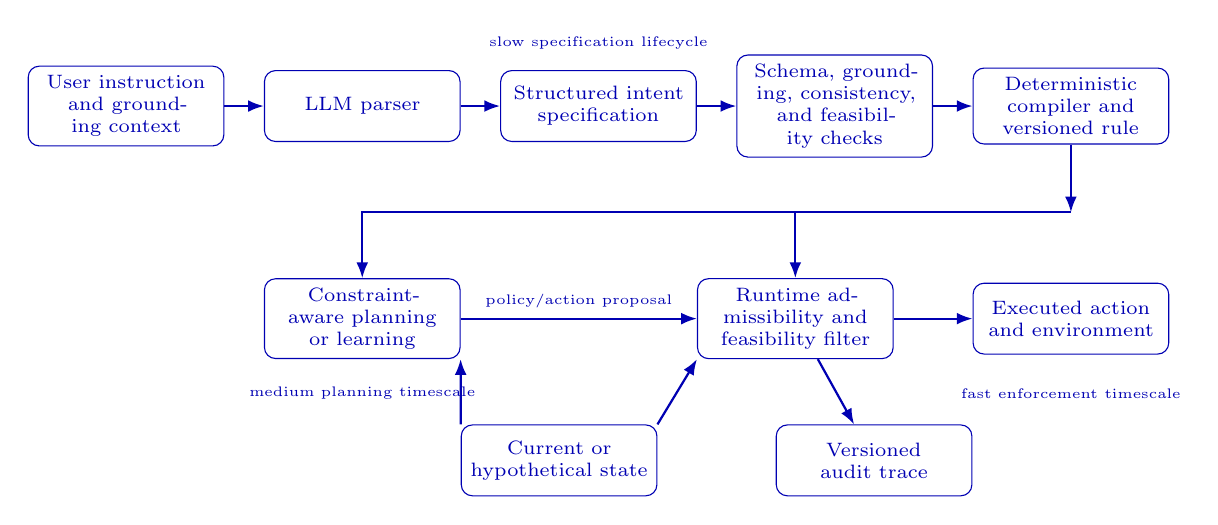
\begin{tikzpicture}[
      node distance=4mm,
      >={Latex[length=2mm]},
      box/.style={draw=blue!70!black, text=blue!70!black, rounded corners,
        align=center, text width=2.25cm, minimum height=9mm, font=\scriptsize},
      flow/.style={->, thick, draw=blue!70!black},
      note/.style={font=\tiny, text=blue!70!black, align=center}]
    \node[box] (user) at (0,0) {User instruction and grounding context};
    \node[box] (parser) at (3,0) {LLM parser};
    \node[box] (spec) at (6,0) {Structured intent specification};
    \node[box] (valid) at (9,0) {Schema, grounding, consistency, and feasibility checks};
    \node[box] (compile) at (12,0) {Deterministic compiler and versioned rule};
    \draw[flow] (user) -- (parser);
    \draw[flow] (parser) -- (spec);
    \draw[flow] (spec) -- (valid);
    \draw[flow] (valid) -- (compile);
    \node[note] at (6,0.8) {slow specification lifecycle};

    \node[box] (plan) at (3,-2.7) {Constraint-aware planning or learning};
    \node[box] (filter) at (8.5,-2.7) {Runtime admissibility and feasibility filter};
    \node[box] (act) at (12,-2.7) {Executed action and environment};
    \node[box] (state) at (5.5,-4.5) {Current or hypothetical state};
    \node[box] (audit) at (9.5,-4.5) {Versioned audit trace};
    \coordinate (branch) at (12,-1.35);
    \draw[flow] (compile.south) -- (branch);
    \draw[flow] (branch) -| (plan.north);
    \draw[flow] (branch) -| (filter.north);
    \draw[flow] (state.north west) -- (plan.south east);
    \draw[flow] (state.north east) -- (filter.south west);
    \draw[flow] (plan) -- node[note, above] {policy/action proposal} (filter);
    \draw[flow] (filter) -- (act);
    \draw[flow] (filter) -- (audit);
    \node[note] at (3,-3.65) {medium planning timescale};
    \node[note] at (12,-3.65) {fast enforcement timescale};
  \end{tikzpicture}
  \caption{\added{Language-to-admissibility architecture. The LLM interprets
  language outside the fast decision loop. A deterministic compiled rule is
  shared by constraint-aware planning and the final runtime filter; executed
  actions and active rule versions are recorded for audit.}}
  \label{fig:lifecycle}
\end{figure}

\begin{minipage}{\linewidth}
\begin{algorithm}[\added{Intent compilation, activation, and constrained execution}]
\label{alg:lifecycle}
\mbox{}\par\smallskip
{\color{blue!70!black}
\begin{enumerate}[leftmargin=*,label=\arabic*.,nosep]
  \item Parse instruction $l$ and grounding context $x$ into a typed
  specification $h=f_\phi(l,x)$.
  \item Validate syntax, types, grounding, consistency, and declared conflict
  semantics; reject or request clarification if validation fails.
  \item Compile $h$ into a reusable predicate $\cI_{\mathrm{new}}(s)$ that can
  be evaluated on observed or hypothetical states.
  \item Check feasibility or viability to the extent supported, then atomically
  activate a versioned compiled rule; do not silently relax an empty set.
  \item Plan or update a proposal policy using
  $\cA_{\cI_{\mathrm{new}}}(s)=\cA_0(s)\cap\cI_{\mathrm{new}}(s)$ in current-
  and successor-state computations.
  \item At each decision, evaluate the active rule on the current state, filter
  the proposal, execute only an admissible action, and log the state, rule
  version, admissible set, proposal, and executed action.
  \item On a new instruction, repeat Steps 1--4; until Step 5 completes, place
  any older or generic proposal policy behind the newly activated filter.
\end{enumerate}}
\end{algorithm}
\end{minipage}
\smallskip

\subsection{\added{Structured Intent and Compilation}}
\label{subsec:parsing}

Let $l \in \cL$ denote a natural-language instruction and let
$x\in\cX$ denote the contextual information needed to ground its entities,
units, and predicates. Let $\mathcal{G}$ be a typed intent-specification
language.

\begin{definition}[Intent Parser]
An \emph{LLM-based intent parser} and an \emph{intent compiler} are mappings
\begin{equation}
  f_\phi : \cL \times \cX \to \mathcal{G},
  \qquad
  g : \mathcal{G}\times\cS\to
  \deleted{2^{\cA}}\hspace{0.25em}\added{\mathcal P(\cA)},
  \qquad
  \cI_{l,x}(s)=g(f_\phi(l,x),s),
  \label{eq:llm_map}
\end{equation}
where $\phi$ denotes the parser parameters. The parser produces a structured
specification, while the compiler evaluates that specification in state $s$
to produce the \deleted{admissible action set}\hspace{0.25em}\added{set permitted by the
compiled intent}.
\end{definition}

\added{Compilation produces a general rule or predicate, not merely a mask over
the actions visible in the state at compilation time. The same artifact must be
evaluable for arbitrary hypothetical states used by a planner and for observed
states encountered during execution. Its intersection with $\cA_0(s)$ changes
the action domain available to optimization; it does not rewrite $R$ or
$\cP$.}

\deleted{For example, consider the instruction}\\
\deleted{\emph{"purchase Product X}}
\deleted{\emph{only from a verified}}
\deleted{\emph{seller without making}}
\deleted{\emph{the remaining budget}}
\deleted{\emph{negative."}}\\
\deleted{In an Agentic Commerce state $s$, let
$\operatorname{verified}(v,s)\in\{0,1\}$ denote the verification status of
seller $v$ and let $b(s)$ denote the remaining authorized budget.}
\deleted{The dependence of $\operatorname{verified}(v,s)$ on $s$ is intentional:
seller eligibility is evaluated from information available in the current
state rather than treated as a permanently fixed property.}
\deleted{For a purchase action $a=\operatorname{buy}(v,X,p)$ for Product X from
seller $v$ at total price $p$, the compiler may define}
\begin{equation}
  \begin{aligned}
  \deleted{a\in\cI_{l,x}(s)}
  &\deleted{\quad\Longleftrightarrow\quad
  \operatorname{verified}(v,s)=1}\\
  &\deleted{\hspace{1.5cm}\land\;p\leq b(s).}
  \end{aligned}
  \label{eq:commerce_intent}
\end{equation}
\deleted{The reward can then optimize price, delivery time, or product quality
among purchase actions in the effective set
$\cA_\cI(s)=\cA_0(s)\cap\cI_{l,x}(s)$.}
\deleted{Equation~\eqref{eq:commerce_intent} assumes that seller verification
and remaining budget are represented in the state.}
\deleted{Identity, delegated payment authorization, checkout, and settlement
remain responsibilities of the surrounding commerce infrastructure rather than
the ICMDP itself.}

\added{For the cloud instruction in Example~\ref{ex:cloud}, the parser may
produce the structured specification}
{\color{blue!70!black}
\[
 G=\left\{
 \begin{array}{ll}
   \textsc{Prohibit:} & \texttt{action = DEPLOY},\\
   \textsc{When:} & \texttt{incident\_severity = SEV1}.
 \end{array}\right.
\]}
\added{Conceptually, the language and compiler stages satisfy}
{\color{blue!70!black}
\begin{equation}
 f_\phi(l,x)\longrightarrow G,
 \qquad
 g(G,s)\longrightarrow\cI_{\mathrm{sev1}}(s).
 \label{eq:cloud_compiler}
\end{equation}}
\added{The artifact $G$ denotes the general predicate in
Equation~\eqref{eq:cloud_intent}, not a list of actions permitted only in the
state observed during parsing. The compiler can therefore evaluate the same
rule in a current state or in hypothetical future states considered by a
planner. Reward optimization then trades service availability, latency,
recovery time, and infrastructure cost among actions in
$\cA_0(s)\cap\cI_{\mathrm{sev1}}(s)$.}

The parser $f_\phi$ performs semantic interpretation, not action optimization.
The intermediate language $\mathcal G$ permits schema and consistency checks
before the deterministic compiler $g$ is admitted to the action-selection
path. The ICMDP optimization~\eqref{eq:icmdp_bellman} then operates over the
\deleted{compiled set}\hspace{0.25em}\added{effective admissible set}. Thus the LLM does not
enforce the constraint; the compiler produces the semantic intent
specification $\cI(s)$, while the action filter enforces $\cA_\cI(s)$. The
parser and compiler can also be revised independently. \added{No LLM call is
required inside a Bellman backup or at each decision step. The trusted
enforcement boundary is the deterministic compiler, active-rule store, and
runtime filter, not the probabilistic language model.}
\tbd{Intent language: define executable syntax and denotational semantics for
$\mathcal G$; typed entities, units, and grounding context $\cX$; supported
statewise and temporal predicates; quantification and composition; defaults,
conflict detection and resolution; versioning; failure semantics; and a
deterministic compilation algorithm $g$ with conformance tests linking each
construct to its state--action predicate.}

\subsection{Validation and Runtime Enforcement}
\label{subsec:enforcement}

Because $f_\phi$ is learned rather than specified by a fixed grammar, it is
subject to misinterpretation. Relative to the user's intended specification,
errors can occur in two directions:
\begin{itemize}[leftmargin=*]
  \item \textbf{Constraint over-tightening.} $f_\phi$ excludes actions the
  user did not intend to exclude, shrinking $\cA_\cI(s)$ and increasing the
  risk that $\cA_\cI(s) = \emptyset$ for some reachable $s$.
  \item \textbf{Constraint under-specification.} $f_\phi$ fails to exclude
  actions the user intended to forbid, so $\cI(s)$ is too permissive and the
  zero-violation guarantee no longer holds with respect to the user's actual
  intent, even though it still holds with respect to the (incorrect)
  extracted $\cI(s)$.
\end{itemize}
\added{These are failures of \emph{specification correctness}: whether the
compiled predicate expresses what the user meant. They are distinct from
\emph{enforcement correctness}: whether the system faithfully applies the
active compiled predicate to every executed action. Runtime filtering can
establish the latter relative to a compiled rule, but cannot establish the
former without additional evidence about interpretation and grounding.}
Either error can change the feasible policy class abruptly. The enforcement
pipeline therefore requires at least: (i) syntax, type,
grounding, and consistency checks on the extracted specification before it is
compiled; (ii) offline reachability or viability analysis when tractable,
combined with a runtime monitor that checks
$\cA_\cI(s_t) \neq \emptyset$ at the current state and triggers safe fallback
or clarification behavior from Section~\ref{subsec:model} when it fails; and
(iii) an audit trace recording,
for each executed action $a_t$, the admissible set $\cA_\cI(s_t)$ it was
drawn from, so that compliance with the extracted intent can be verified
after the fact. The trace records membership in $\cA_\cI(s_t)$, not a
statistical property of the policy. It can therefore support an audit of the
compiled filter, but it does not show that the parsed specification matches
the user's meaning.
\deleted{\textbf{TBD Viability:} develop a forward-looking check that prevents
admissible actions from entering states with no admissible continuation;
current-state nonemptiness alone does not guarantee future feasibility.}
\tbd{Viability: when global feasibility has not been established---for example
under runtime-only feasibility checks, dynamic intent, or richer temporal
constraints---current-state nonemptiness does not by itself establish the
existence of a feasible continuation. Develop an appropriate viability or
reachability condition for these settings.}
\tbd{Verification: define a threat model, trusted computing boundary, log
integrity mechanism, and machine-checkable proof obligations before describing
the audit trace as a formal certificate.}

\subsection{\added{Dynamic Intent Update Protocol}}
\label{subsec:update_protocol}

\added{Section~\ref{subsec:extensions} distinguishes the mathematical cases
for changing intent. Operationally, a new instruction is parsed and validated
without modifying the active rule. The candidate rule is compiled under a new
version, checked for current-state nonemptiness and any available forward
feasibility condition, and then activated atomically. A failed candidate leaves
the previous rule active and triggers clarification or escalation; it is not
partially installed. Once activation succeeds, the runtime filter applies the
new rule at the next action-selection boundary. Policy recomputation may then
proceed asynchronously. This ordering separates immediate enforcement of the
compiled update from the longer task of recovering optimal behavior under the
new admissible domain. In the cloud example, the deployment-freeze rule
$\cI_2$ in Equation~\eqref{eq:deployment_freeze} replaces the conditional Sev1
rule $\cI_1$ only after this activation step; subsequent actions are filtered
under $\cI_2$ while policy adaptation proceeds.}

% -----------------------------------------------------------------------
\section{Solution Methods and Analysis}
\label{sec:algorithms}
% -----------------------------------------------------------------------

ICMDP changes the feasible action set rather than the reward or cost
functions. \deleted{Standard dynamic-programming and reinforcement-learning
algorithms therefore apply after inadmissible actions are removed from policy
evaluation and improvement.}\hspace{0.25em}\added{Constraint-aware planning
therefore applies the compiled predicate throughout policy evaluation,
improvement, Bellman backups, and learning targets: admissibility is evaluated
at both current and hypothetical successor states. A final runtime filter
independently enforces the active rule on the action actually executed.}

\subsection{Intent-Filtered Planning and Learning}
\label{subsec:planning}

\deleted{Planning and enforcement are complementary. Suppose action $a$ at
$s_0$ leads to $s_1$, where a generic planner expects to take a high-value
action $b$, but $b\notin\cA_\cI(s_1)$. A runtime filter at $s_1$ prevents
execution of $b$ and thereby preserves compliance, yet a planner that ignored
future admissibility may still have selected $a$ on the basis of an unavailable
continuation. Constraint-aware planning evaluates $a$ using
$\max_{a'\in\cA_\cI(s_1)}Q(s_1,a')$ and can instead prefer an admissible route
from $s_0$.}
\added{Planning and enforcement are complementary in the cloud example.
Suppose an action at $s_0$ can lead to a future Sev1 state $s_1$. An
unconstrained planner may value that action while assuming that
$\operatorname{Deploy}$ will remain available at $s_1$. The runtime filter
prevents deployment after $s_1$ is reached, but it does not correct the earlier
valuation at $s_0$. Constraint-aware planning instead computes
$V_\cI^*(s_0)$ using the restricted future set
$\cA_\cI(s_1)$ and can prefer a trajectory with a better admissible
continuation.} Runtime filtering guarantees membership of the executed action;
it does not by itself produce a policy optimal for the restricted problem.

\paragraph{Value iteration.}
Value iteration restricts the Bellman update~\eqref{eq:icmdp_bellman}:
\begin{equation}
  V_{k+1}(s) = \max_{a \in \cA_\cI(s)}\left[R(s,a) + \gamma
  \sum_{s' \in \cS} \cP(s' \given s, a)\, V_k(s')\right].
  \label{eq:intent_vk}
\end{equation}
The restriction to $\cA_\cI(s)$ is state-dependent action masking before the
Bellman backup \citep{huang2022}.

\paragraph{Policy iteration.}
Policy evaluation is unchanged but applied to an admissible policy
$\pi \in \Pi_\cI$. Define
\[
  Q^\pi(s,a)\coloneqq R(s,a)+\gamma\sum_{s'\in\cS}
  \cP(s'\given s,a)V^\pi(s').
\]
Policy improvement selects a deterministic admissible decision rule,
\begin{equation}
  \mu_{k+1}(s) \in \argmax_{a \in \cA_\cI(s)} Q^{\pi_k}(s,a)
  \quad \forall\, s \in \cS.
\end{equation}
The induced policy places unit mass on $\mu_{k+1}(s)$. For a directly specified
admissible set, no Lagrangian relaxation is required; compliance with the
\deleted{compiled set}\hspace{0.25em}\added{effective admissible set} follows by construction
of $\Pi_\cI$.

\paragraph{Model-free learning.}
\deleted{In model-free settings, ICMDP can be implemented via action masking in
Q-learning and policy-gradient algorithms. Let
$\mathcal{M}(s,a) \in \{0,1\}$ denote the action-masking function, equal to
$1$ iff $a \in \cA_\cI(s)$.}\hspace{0.25em}
\added{In model-free settings, the admissible set $\cA_\cI(s)$ can be enforced
through action masking in Q-learning and policy-gradient algorithms.}
Both the behavior policy used for exploration and
the next-state bootstrap must be restricted to the admissible sets. For a
sampled admissible action, the update is
\begin{equation}
  Q(s,a) \leftarrow Q(s,a) + \alpha\!\left[R(s,a)
    + \gamma \max_{a' \in \cA_\cI(s')} Q(s',a') - Q(s,a)\right],
  \quad a \in \cA_\cI(s),
\end{equation}
and for policy gradient methods, masked logits $z_\theta(s,a)$ yield
\begin{equation}
  \pi_\theta(a \given s) =
  \begin{cases}
    \dfrac{\exp\bigl(z_\theta(s,a)\bigr)}
          {\displaystyle\sum_{a' \in \cA_\cI(s)} \exp\bigl(z_\theta(s,a')\bigr)}
    & \text{if } a \in \cA_\cI(s), \\[8pt]
    0 & \text{otherwise,}
  \end{cases}
  \label{eq:masked_policy}
\end{equation}
This is equivalent to setting inadmissible logits to $-\infty$ before the
softmax and gives them zero probability \citep{huang2022}. \added{Thus the
masked distribution is the executed or effective policy. Sampling for
exploration uses the current-state mask, the bootstrap target uses the
successor-state mask, and policy-gradient log-probability and entropy terms are
computed from the masked distribution during training as well as execution.}
\tbd{Model-free theory: add a primary reference and state convergence
conditions for masked Q-learning; \deleted{Theorem}\hspace{0.25em}\added{Proposition}~\ref{thm:contraction} establishes
value-iteration convergence, not convergence under function approximation.}

\subsection{Computational and Robustness Analysis}
\label{subsec:analysis}

\paragraph{Convergence and complexity.}
\deleted{Theorem}\hspace{0.25em}\added{Proposition}~\ref{thm:contraction} gives convergence of
\eqref{eq:intent_vk}. With an
explicit transition model, the per-iteration backup cost is
\[
  O\!\left(\sum_{s\in\cS}\sum_{a\in\cA_\cI(s)}
  |\operatorname{supp}\cP(\cdot\given s,a)|\right),
\]
plus the cost of evaluating or retrieving each admissible set. Small admissible
sets reduce Bellman-backup work. \deleted{although an online LLM call may
dominate this saving. Parsing once and caching or incrementally evaluating the
compiled specification avoids repeated calls when the instruction is
unchanged.}\hspace{0.25em}\added{The costs occur on three timescales: language
parsing, validation, and compilation on the slow specification timescale;
policy computation or adaptation on the medium planning timescale; and
deterministic predicate evaluation, filtering, and logging on the fast
enforcement timescale. Because the LLM is outside the fast loop, its latency
affects instruction updates rather than every Bellman backup or action.}

\paragraph{Comparison to CMDP solvers.}
Many CMDP solvers use Lagrangian dual optimization and iterative multiplier
updates. When intent is represented directly as an admissible set, ICMDP can
instead use ordinary restricted-action dynamic programming. Proposition
\ref{prop:cmdp_encoding} shows that this is a representational and algorithmic
distinction, not a blanket claim of greater expressive power.

\paragraph{Empty feasible sets.}
\deleted{If $\cI$ is overly restrictive,}\hspace{0.25em}
\added{If operational availability or compiled intent leaves}
$\cA_\cI(s) = \emptyset$ for some reachable
$s$ and~\eqref{eq:icmdp_bellman} is undefined there (Definition
\ref{def:feasibility}). Any implementation must therefore include a
feasibility monitor that checks $\cA_\cI(s_t) \neq \emptyset$ before action
selection and triggers a predefined safe fallback, termination, or user
clarification when it fails, as described in Section~\ref{subsec:model}. This
\deleted{local check does not by itself prevent a currently admissible action
from leading to a future state with no admissible continuation.}\hspace{0.25em}
\added{When only local runtime feasibility is available rather than the global
condition of Definition~\ref{def:feasibility}, current-state nonemptiness does
not by itself establish a feasible continuation.}

\paragraph{Changing constraints.}
\deleted{Dynamic intent (Section~\ref{subsec:extensions}) breaks the stationarity
assumption underlying~\eqref{eq:intent_vk}. In practice this requires either
re-running value iteration after each constraint update or maintaining
incremental value estimates that are corrected as $\cI_t$ changes; efficient
incremental algorithms for this setting are an open problem.}
\added{An exogenous change to $\cI_t$ breaks the stationarity assumption
underlying~\eqref{eq:intent_vk} and may require replanning or incremental policy
adaptation. It does not require the system to postpone compliance until such
optimization completes: after the validation and atomic activation protocol in
Section~\ref{subsec:update_protocol}, the new rule is applied by the runtime
filter at the next action-selection boundary. A time-homogeneous augmented-state
model permits stationary methods on a larger state space. The computational and
performance implications of these alternatives remain open. In particular, the
deployment freeze in Equation~\eqref{eq:deployment_freeze} can be enforced
before a policy optimized for $\cI_1$ has been adapted to $\cI_2$.}
\tbd{Dynamic intent: define the update protocol, consistency semantics, and
regret or convergence objective for non-stationary admissible sets.}

\paragraph{Parser over- and under-restriction.}
The two failure directions identified in Section~\ref{subsec:enforcement}
have distinct algorithmic consequences: over-tightening manifests as spurious
infeasibility (handled by the feasibility monitor above), while
under-specification manifests as silent non-compliance with the user's
actual intent, which no amount of downstream planning can detect without an
independent verification step against the original instruction $l$.

% -----------------------------------------------------------------------
\section{Discussion}
\label{sec:discussion}
% -----------------------------------------------------------------------

\subsection{Relationship to CMDP, RLHF, and Action Masking}
\label{subsec:relationship}

Table~\ref{tab:comparison} compares
RLHF, CMDP, and ICMDP. RLHF modifies the reward function
\citep{christiano2017}; CMDP constrains expected cumulative cost
\citep{altman1999}; ICMDP constrains the admissible action space directly.
The methods are compatible: RLHF or a
CMDP objective can optimize qualitative or budget-level behavior \emph{within}
the admissible region $\cA_\cI(s)$ that ICMDP defines. Action masking and shielding
(Section~\ref{subsec:related}) share ICMDP's hard, per-step mechanism but are
typically driven by hand-written rules. In the proposed pipeline, the parser
in Section~\ref{sec:llm} derives the admissibility function from natural
language.

\added{Constraint-aware planning and runtime enforcement serve different
purposes. The planner anticipates present and future admissibility when
optimizing return and can avoid trajectories with poor or infeasible
continuations. The runtime filter protects the final execution boundary against
stale policies, approximation error, or delayed replanning. Planning without a
final filter weakens enforcement assurance; filtering without constrained
planning can remain compliant while sacrificing substantial return. The
normal-to-Sev1 transition in Section~\ref{subsec:planning} illustrates this
distinction within the running cloud-operations scenario.}

\begin{table}[ht]
  \centering
  \caption{Representational comparison. Guarantees in every column are
  conditional on the correctness of the corresponding learned or formal
  specification and its implementation.}
  \label{tab:comparison}
  \small
  \begin{tabular}{>{\raggedright\arraybackslash}p{2.5cm}
                  >{\raggedright\arraybackslash}p{3.0cm}
                  >{\raggedright\arraybackslash}p{3.0cm}
                  >{\raggedright\arraybackslash}p{3.0cm}}
    \toprule
    Property & RLHF & CMDP & ICMDP \\
    \midrule
    Primary representation &
      Learned preference reward &
      Expected cumulative costs and thresholds &
      Statewise admissible-action set \\
    Enforcement point &
      Reward optimization &
      Policy-level feasibility constraint &
      Action-selection filter \\
    Exclusion guarantee &
      None from the reward model alone &
      Possible for nonnegative violation cost with zero budget &
      Zero policy mass on compiled exclusions \\
    Cumulative budgets &
      Indirectly through reward design &
      Native &
      Requires augmented state or a separate constraint mechanism \\
    Natural-language input &
      Preference data or language-dependent reward model &
      Requires cost/threshold translation &
      \deleted{Parsed, validated, and compiled into $\cI$}
      \added{Parsed, validated, and compiled into $\cI$; intersected with
      $\cA_0(s)$ to form $\cA_\cI(s)$} \\
    \bottomrule
  \end{tabular}
\end{table}

\subsection{Scope of the Guarantee}
\label{subsec:guarantees}

Given \deleted{a correctly specified $\cI$}\hspace{0.25em}\added{correctly specified
$\cA_0$ and $\cI$}, every policy in $\Pi_\cI$ assigns zero
probability to inadmissible actions by construction
(Section~\ref{subsec:model}), not by statistical estimation. This statement
depends on \deleted{three}\hspace{0.25em}\added{four} assumptions from
Section~\ref{subsec:model}: the true state (or an exact sufficient statistic)
is observed, \added{$\cA_0$ correctly represents operational availability,}
$\cI$ is derived correctly from the user's instruction, and the
ICMDP is \deleted{intent-feasible}\hspace{0.25em}\added{globally intent-feasible}.

\added{For exogenous dynamic intent, the same statement is version-relative:
after a validated rule $\cI_t$ is atomically activated, the executed policy
assigns zero probability to actions outside $\cA_0(s)\cap\cI_t(s)$ at subsequent
action-selection boundaries. This claim assumes correct activation, state
information, predicate evaluation, and filtering. It neither applies
retroactively nor implies that a policy awaiting reoptimization is optimal for
the revised admissible domain.}

Each assumption may fail in practice:

\paragraph{Parsing errors.}
Section~\ref{subsec:enforcement} identified over-tightening and
under-specification as the two failure directions of $f_\phi$. Constraint
errors produce hard exclusions or hard omissions and can therefore alter the
feasible policy class discontinuously. Reward-model errors can also be severe;
the distinction is structural rather than a claim that one error source always
degrades more gracefully than the other.

\paragraph{Partial observability.} The present formulation assumes state
observability. A belief-dependent
admissibility function $\cI(b)$---conditioning intent on a belief state
rather than the true state---is left for future work.
\tbd{Partial observability: define belief-dependent, robust, or
chance-constrained admissibility and prove the corresponding guarantee before
claiming support for POMDPs.}

\paragraph{Scalability.} The pipeline invokes an LLM for intent parsing and,
potentially, for periodic re-validation as constraints change
(Section~\ref{subsec:extensions}). Model latency can be a bottleneck for
real-time deployment; caching
and intent pre-compilation can mitigate it but trade off against how quickly
the system can react to a genuinely new instruction.

\paragraph{Absence of empirical evaluation.}
The paper contains no quantitative comparison of policy performance, empirical
solver study, or evaluation of noisy intent extraction. The formal results
hold under their stated assumptions but do not establish performance in a
deployed system. In particular, the \deleted{Agentic Commerce mapping in
Section~\ref{subsec:parsing} is illustrative and has not
been evaluated in a live commerce or payment workflow.}
\added{cloud-operations scenario in Example~\ref{ex:cloud} is an explanatory
model and has not been evaluated in a production control plane.}
\tbd{Evaluation protocol: report specification accuracy separately from
enforcement accuracy, including exact predicate equivalence where ground truth
is available, over- and under-restriction rates, action-level violations,
return, infeasibility, clarification frequency, update latency, filter latency,
and audit completeness. Compare unconstrained planning, reward penalties,
runtime-only filtering, planning-only masking, and combined planning plus
runtime enforcement \deleted{under clean, ambiguous, and deliberately perturbed
instructions}\hspace{0.25em}\added{in a small simulated cloud-control MDP with
normal, degraded, and Sev1 states; deployment, rollback, restart, scaling, and
no-operation actions; clean, ambiguous, and deliberately perturbed
instructions; and the mid-execution deployment-freeze update}.}

% -----------------------------------------------------------------------
\section{Conclusion}
\label{sec:conclusion}
% -----------------------------------------------------------------------

\deleted{ICMDP represents a compiled intent specification as the admissible
action set of an MDP.}\hspace{0.25em}\added{This paper presents ICMDP as a
language-to-admissibility framework: baseline operational availability is
intersected with a validated, compiled intent rule to form the effective action
domain used by planning and runtime enforcement.} We derived the restricted
Bellman equations and feasibility conditions, \deleted{proved contraction and
convergence of the Bellman operator,}\hspace{0.25em}\added{stated the standard
contraction and convergence properties inherited under fixed admissibility,}
and gave standard dynamic-programming and model-free implementations over the
restricted action set. Proposition~\ref{prop:cmdp_encoding} shows that statewise
exclusions also admit a zero-budget CMDP encoding along reachable trajectories;
ICMDP's distinction is therefore its explicit lifecycle from language through
structured specification, validation, compilation, constraint-aware planning,
runtime filtering, dynamic activation, and audit---not a new Bellman theory or
a blanket expressiveness advantage. The parser--compiler separation also
exposes failure modes including over-tightening, under-specification, empty
feasible sets, and changing intent.

\added{The cloud-operations example demonstrates this lifecycle with one fixed
Sev1 deployment rule and one genuine deployment-freeze update. It is an
expository instance rather than a domain-specific contribution; the formal
interface remains applicable to other sequential agent systems.}

The immediate next step is to evaluate computational feasibility and
robustness to parsing errors in a reproducible implementation. Open theoretical
questions include (i) efficient online algorithms for changing intent
constraints, (ii) formal verification of LLM-derived intent mappings prior to
policy optimization, (iii) a belief-dependent extension of $\cI$ for
partially observable settings, and (iv) hybrid architectures in which RLHF or
a CMDP objective optimizes qualitative behavior within the feasible region
that ICMDP defines.
\deleted{Paper identity: after completing the literature review and evaluation,
decide whether to present the final manuscript primarily as a formal theory
paper or as a language-to-enforcement framework paper, and revise title,
abstract, and contribution claims consistently.}\hspace{0.25em}
\added{The present revision adopts the language-to-enforcement framework
positioning consistently while retaining the formal model needed to state its
interface and conditional guarantees.}

% -----------------------------------------------------------------------
%  Bibliography
% -----------------------------------------------------------------------
\bibliographystyle{plainnat}
\bibliography{references}

\end{document}
